% generated by plots/fig9_trajectories.py --- do not edit the numbers by hand
% figure* --- the chapter is two-column and this does not fit one
\begin{figure}[tp]
\centering
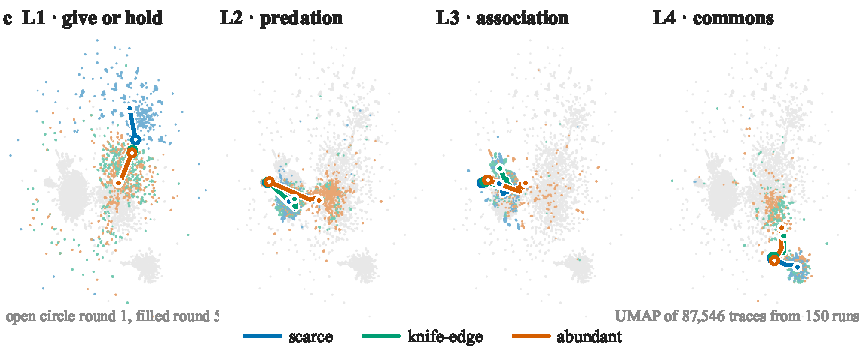
\includegraphics[width=\linewidth]{figures/fig9_trajectories/trajectories.pdf}\\[2pt]
\caption[Reasoning traces projected, by capacity level]{%
\textbf{Reasoning traces projected, by capacity level.} The 87,546 reasoning traces of the 150 production runs, projected to two dimensions, one panel per capacity level. Grey is every trace in the study and the tinted points are that panel's own; the line is the mean position of a payoff cell at each sampled round, from an open circle at the first to a filled one at the last. Distances on the page carry no unit, since the projection preserves neighbourhoods while it is free to stretch everything else. Nothing here is a test.}
\label{fig:trajectories}
\end{figure}
